\documentclass[a4paper,12pt]{article}
\usepackage[a4paper,top=1.3cm,bottom=2cm,left=1.5cm,right=1.5cm,marginparwidth=0.75cm]{geometry}
%%% Работа с русским языком
\usepackage{cmap}					% поиск в PDF
\usepackage{mathtext} 				% русские буквы в фомулах
\usepackage[T1, T2A]{fontenc}			% кодировка
\usepackage[utf8]{inputenc}			% кодировка исходного текста
\usepackage[english,russian]{babel}	% локализация и переносы

\usepackage{graphicx}

\usepackage{wrapfig}
\usepackage{tabularx}

\usepackage{hyperref}
\usepackage[rgb]{xcolor}
\hypersetup{
colorlinks=true,urlcolor=blue
}

%%% Дополнительная работа с математикой
\usepackage{amsmath,amsfonts,amssymb,amsthm,mathtools}
\usepackage{icomma} % "Умная" запятая: $0,2$ --- число, $0, 2$ --- перечисление

%% Номера формул
\mathtoolsset{showonlyrefs=true} % Показывать номера только у тех формул, на которые есть \eqref{} в тексте.

%% Шрифты
\usepackage{euscript}	 % Шрифт Евклид
\usepackage{mathrsfs} % Красивый матшрифт

%% Свои команды
\DeclareMathOperator{\sgn}{\mathop{sgn}}

%% Перенос знаков в формулах (по Львовскому)
\newcommand*{\hm}[1]{#1\nobreak\discretionary{}
{\hbox{$\mathsurround=0pt #1$}}{}}

%%% Заголовок
\author{Волков Никита Алексеевич}
\title{Лабораторная работа №1.1.1

Измерение удельного сопротивления нихромовой проволоки
}
\date{\today}

\begin{document}

\begin{titlepage}
	\begin{center}
		{\large МОСКОВСКИЙ ФИЗИКО-ТЕХНИЧЕСКИЙ ИНСТИТУТ (НАЦИОНАЛЬНЫЙ ИССЛЕДОВАТЕЛЬСКИЙ УНИВЕРСИТЕТ)}
	\end{center}
	\begin{center}
		{\large Физтех-школа аэрокосмических технологий}
	\end{center}
	
	
	\vspace{4.5cm}
	{\huge
		\begin{center}
			{\bf Отчёт о выполнении лабораторной работы 1.1.1}\\
			Определение систематических и случайных погрешностей при измерении удельного сопротивления нихромовой проволоки
		\end{center}
	}
	\vspace{2cm}
	\begin{flushright}
		{\LARGE Автор:\\ Волков Никита Алексеевич \\
			\vspace{0.2cm}
			Б03-103}
	\end{flushright}
	\vspace{8cm}
	\begin{center}
		Долгопрудный 2021
	\end{center}
\end{titlepage}

\tableofcontents

\newpage

\section{Введение}

\textbf{Цель работы:} измерить удельное сопротивление проволоки и вычислить систематические и случайные погрешности при использовании таких измерительных приборов, как линейка, штангенциркуль, микрометр, амперметр, вольтметр и мост постоянного тока.
\medskip

\textbf{В работе используются:} линейка, штангенциркуль, микрометр, отрезок проволоки из нихрома, амперметр, вольтметр, источник ЭДС, мост постоянного тока, реостат, ключ.
\medskip

В работе используются следующие методы измерения сопротивления:
\begin{enumerate}
	\item определение углового коэффициента наклона зависимости напряжения на проволоке от тока через неё;
	\item измерение с помощью моста постоянного тока.
\end{enumerate}


\section{Теоретические сведения}

Удельное сопротивления однородной проволоки круглого сечения можно определить по следующей формуле:

\begin{equation}\label{ydelnoe_soprotivlenie}
\rho = \frac{R_{\text{пр}}}{l}\frac{\pi d^2}{4},
\end{equation}

\noindent где $R_{\text{пр}}$ -- сопротивление проволоки, $d$ -- её диаметр, $l$ -- длина.


Диаметр проволоки немного меняется по длине случайным образом, поэтому в формулу \eqref{ydelnoe_soprotivlenie} необходимо подставлять среднее по длине значение диаметра и учитывать соответствующую случайную погрешность этого значения.


\begin{wrapfigure}{r}{0.5\textwidth}
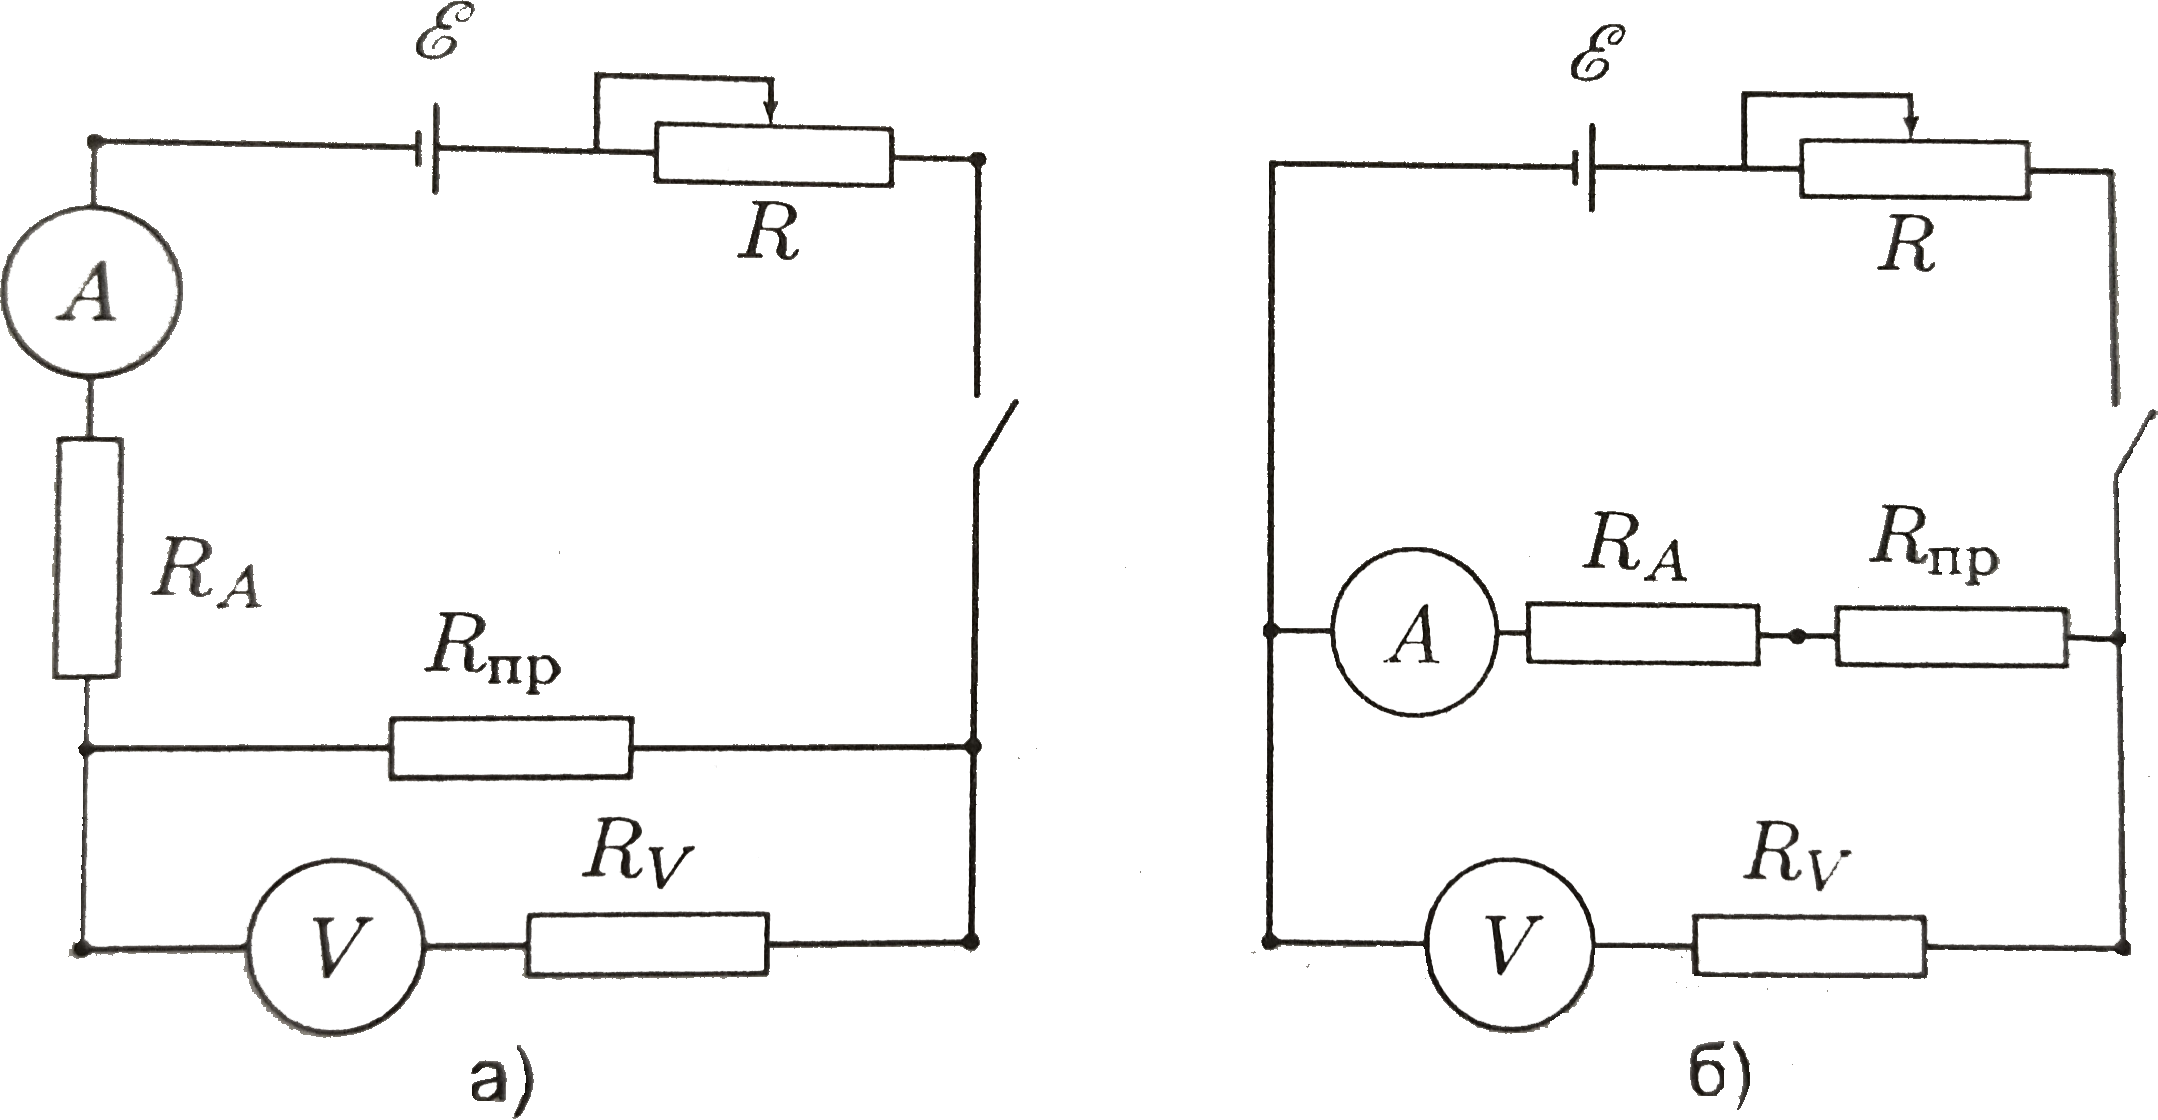
\includegraphics[width=0.5\textwidth]{schemi}
\caption{Схемы для измерения сопротивления при помощи амперметра и вольтметра} \label{schemi}
\end{wrapfigure}

Сопротивление $R_{\text{пр}}$ можно измерить с помощью одной из схем, представленных на рис.\ref{schemi}. Здесь $R$ - реостат, $R_A$ - сопротивление амперметра, $R_V$ - сопротивление вольтметра, $R_{\text{пр}}$ - сопротивление исследуемой проволоки.


Пусть $V$ и $I$ - показания вольтметра и амперметра соответственно. По закону Ома можно рассчитать сопротивление проволоки $R_{\text{пр1}} = V_{\text{а}}/I_{\text{а}}$ для схемы (а) и $R_{\text{пр2}} = V_{\text{б}}/I_{\text{б}}$ для схемы (б). Эти величины будут отличаться друг от друга и реального $R_{\text{пр}}$ из-за влияния внутренних сопротивлений приборов.


Учитывая внутреннее сопротивление приборов получаем следующие формулы рассчета сопротивления
Для схемы (а):

\[ R_{\text{пр1}} =\dfrac{V_{\text{а}}}{I_{\text{а}}} = R_{\text{пр}}\dfrac{R_V}{R_{\text{пр}} + R_V} \]

Преобразуем
\begin{equation}\label{Rpr_1}
R_{\text{пр}} = R_{\text{пр1}}\dfrac{R_V}{R_V - R_{\text{пр1}}} = \dfrac{R_{\text{пр1}}}{1 - R_{\text{пр1}}/R_V} \thickapprox R_{\text{пр1}} (1 + \dfrac{R_{\text{пр1}}}{R_V})
\end{equation}


Для схемы (б):

\[ R_{\text{пр2}} =\dfrac{V_{\text{б}}}{I_{\text{б}}} = R_{\text{пр}} + R_A \]

Преобразуем
\begin{equation}\label{Rpr_2}
R_{\text{пр}} = R_{\text{пр2}}(1 - \dfrac{R_A}{R_{\text{пр2}}})
\end{equation}


Члены, стоящие в скобках в формулах \eqref{Rpr_1} и \eqref{Rpr_2}, определяют поправки, которые необходимо внести в измерения. В работе выберем схему, которая приводит к меньшей поправке.


Более точным методом измерения сопротивлений является классический метод моста постоянного тока (мост Уитстона. Для контрольного измерения сопротивления проволоки используем мост Р4833.


\section{Оборудование и эксперементальные погрешности}

\textbf{Линейка:} $\Delta_\text{лин} = \pm 0,5$ мм \\
\textbf{Штангенциркуль:} $\Delta_\text{шт} = \pm 0,05$ мм \\
\textbf{Микрометр:} $\Delta_\text{мкм} = \pm 0,01$ мм \\
\textbf{Вольтметр:} 

\begin{tabular}[]{|l|l|}
\hline
Система & Магнито-электрическая \\
\hline
Класс точности & 0,5 \\
\hline
Предел измерений & 750 мВ  \\
\hline
Цена деления & $5 \cdot 10^{-3} \text{ В} = 5 \text{ мВ}$  \\
\hline
Чувствительность& 150 дел./В \\
\hline
Внутреннее сопротивление& 5 кОм  \\
\hline
Погрешность при считывании со шкалы& $\pm2,5\text{ мВ}$  \\
\hline
Максимальная погрешность по классу точности& $\pm3,75\text{ мВ}$ \\
\hline
\end{tabular}\\

\noindent \textbf{Амперметр:}

\begin{tabular}{|l|l|}
	\hline
	Система&Цифровая \\
	\hline
	Предел измерения&2 А \\
	\hline
	Разрядность дисплея& 5 ед. \\
	\hline
	Внутреннее сопротивление& $R_A = 1,2 \text{ Ом}$ \\
	\hline
\end{tabular}\\

\medskip

\noindent\textbf{Мост постоянного тока P4833:}\\
\begin{tabular}{|p{8cm}|p{7cm}|}
	\hline
	Класс точности&0,1 \\
	\hline
	Разрядность магазина сопротивлений& 5 ед. \\
	\hline
	Исследуемый диапазон измерений& $ 10^{-4} - 10 \text{ Ом} $ (для множителя $ N = 10^{-2} $) \\
	\hline
	Погрешность измерений в используемом диапазоне& $\pm0,010\text{ Ом}$ \\
	\hline
\end{tabular}\\

\medskip

Взяв $R_{\text{пр}} \thickapprox 5 Ом$, $R_A = 1,2 Ом$ и $R_V = 5\cdot10^3 Ом$, рассчитаем относительную поправку к сопротивлению согласно формулам \eqref{Rpr_1} и \eqref{Rpr_2}: \\
для схемы рис.\ref{schemi} а $R_{\text{пр1}}/R_{\text{V}} = 5/5000 = 0,001$ т.е $0,1\%$; \\
для схемы рис.\ref{schemi} б $R_{\text{A}}/R_{\text{пр2}} = 1,2/5 = 0,24$ т.е $24\%$. \\
Меньшую ошибку при малых сопротивлениях проволоки дает схема рис.\ref{schemi}а, поэтому использовать в работе будем ее.

\newpage

\section{Результаты измерений и обработка данных}

\subsection{Измерение диаметра $d$ проволоки}

Измерения проводились штангенциркулем и микрометром для $N = 10$ различных участков проволоки. При измерении штангенциркулем получено $d = 0,4$ мм для всех участков. При измерении микрометром были получены следующие показания:

\begin{table}[h]
	\begin{center}
		\caption{\textit{Измерение диаметра проволоки микрометром}}
		\begin{tabular}{|l|l|l|l|l|l|l|l|l|l|l|}
			\hline
		Номер   измерения & 1    & 2    & 3    & 4    & 5    & 6    & 7    & 8    & 9    & 10   \\ \hline
		d, мм             & 0,37 & 0,37 & 0,37 & 0,37 & 0,37 & 0,36 & 0,36 & 0,37 & 0,37 & 0,37 \\ \hline
		\end{tabular}
	\end{center}
\end{table}

Среднее значение диаметра $ \overline{d} = \frac{\sum d_i}{N} = 0,368 \text{ мм}$.\\

Случайная погрешность измерения $ \sigma_{\overline{d}} = \sqrt{\frac{1}{N  (N-1)}\sum(d_i-\overline{d})^2} \approx 0,001 \text{ мм}$.\\

С учётом инструментальной погрешности $ \Delta_\text{мкм} = 0,005$ мм погрешность диаметра может быть вычислена как $ \sigma^{\text{полн}}_{\overline{d}} = \sqrt{\sigma^2_{\overline{d}} + \Delta^2_{\text{мкм}}} \approx 0,005 \text{ мм}$. \\

\textit{Окончательные результаты измерения диаметра проволоки:}

\begin{itemize}
	\item Штангенциркулем: $ d = 0,40 \pm 0,05 \text{ мм}  $
	\item Микрометром:  $ \underline{0,368 \pm 0,005 \text{ мм}} \left(\varepsilon \thickapprox 1,4 \%\right)  $
\end{itemize}


\subsection{Измерение сопротивления проволоки}

Результаты измерений зависимостей показания вольтметра $ V_\text{В} $ от показаний амперметра $ I_A $ в схеме на рис.\ref{schemi}(а) представлены в таблицах \ref{l20}, \ref{l30}, \ref{l50}. Соответствующие графики зависимостей изображены на рис\ref{graph}.

\begin{table}[h]
\caption{\textit{Показания вольтметра и амперметра для $l = 20 \text{см}$}}
\label{l20}
	\begin{tabular}{|l|l|l|l|l|l|l|l|l|l|l|l|l|l|l|l|l|}
	\hline
	\multicolumn{17}{|c|}{l = 20 см}                                                                         	\\ \hline
	Vв, дел & 139 & 120 & 103 & 86  & 70  & 53  & 39  & 25  & 29  & 36  & 44  & 53  & 61  & 69  & 86  & 103 \\ \hline
	Vв, мВ  & 695 & 600 & 515 & 430 & 350 & 265 & 195 & 125 & 145 & 180 & 220 & 265 & 305 & 345 & 430 & 515 \\ \hline
	Iа, мА  & 340 & 295 & 252 & 209 & 172 & 131 & 96  & 63  & 70  & 90  & 110 & 130 & 150 & 170 & 210 & 252 \\ \hline
	\end{tabular}
\end{table}


\begin{table}[h]
\caption{\textit{Показания вольтметра и амперметра для $l = 30 \text{см}$}}
\label{l30}
	\begin{tabular}{|l|l|l|l|l|l|l|l|l|l|l|l|l|l|}
	\hline
	\multicolumn{14}{|c|}{l = 30 см}                                                       	\\ \hline
	Vв, дел & 142 & 124 & 106 & 88  & 71  & 54  & 35  & 45  & 62  & 81  & 99  & 121 & 139 \\ \hline
	Vв, мВ  & 710 & 620 & 530 & 440 & 355 & 270 & 175 & 225 & 310 & 405 & 495 & 605 & 695 \\ \hline
	Iа, мА  & 240 & 208 & 180 & 149 & 121 & 90  & 60  & 75  & 105 & 136 & 166 & 203 & 233 \\ \hline
	\end{tabular}
\end{table}


\begin{table}[h]
\caption{\textit{Показания вольтметра и амперметра для $l = 50 \text{см}$}}
\label{l50}
	\begin{tabular}{|l|l|l|l|l|l|l|l|l|l|l|}
	\hline
	\multicolumn{11}{|c|}{l = 50 см}                                     \\ \hline
	Vв, дел & 54  & 75  & 99  & 120 & 139 & 130 & 109 & 89  & 70  & 59  \\ \hline
	Vв, мВ  & 270 & 375 & 495 & 600 & 695 & 650 & 545 & 445 & 350 & 295 \\ \hline
	Iа, мА  & 55  & 76  & 100 & 121 & 141 & 131 & 110 & 90  & 71  & 60  \\ \hline
	\end{tabular}
\end{table}


\begin{figure}[h!]
	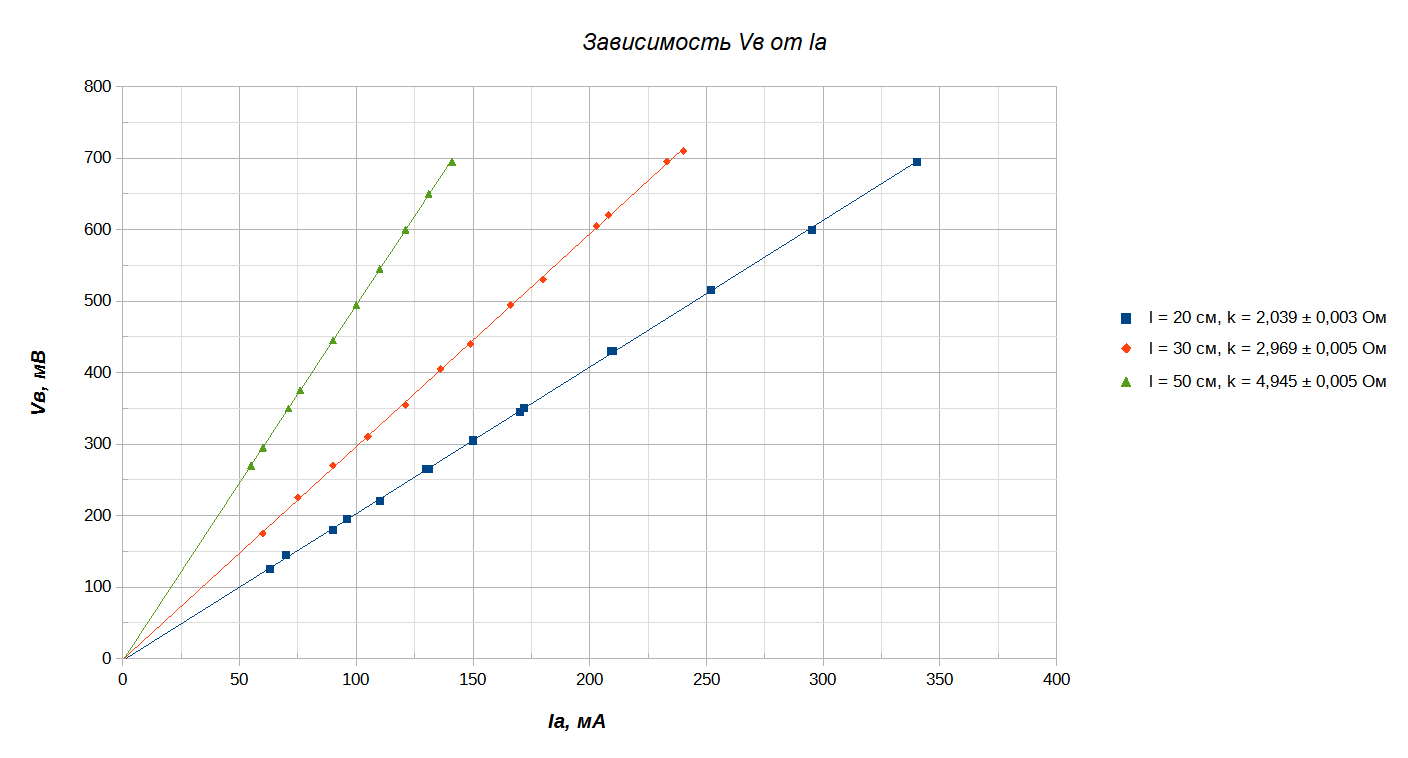
\includegraphics[width=1\linewidth]{graphik-2.png}
	\caption{\textit{Результаты измерений напряжения $ V_\text{В} $ в зависимости от тока $ I_A $ для проволок разной длины $ l $ и их линейная аппроксимация $ y=kx $.}}
	\label{graph}
\end{figure}


\newpage

Пользуясь методом наименьших квадратов, строим аппроксимирующие прямые $ V_\text{В} = \overline{R}I_A $, определяя их угловой коэффициент по формуле

\begin{equation}
\overline{R} = \frac{\langle VI \rangle}{\langle I^2 \rangle}.
\end{equation}

Случайную погрешность определения углового коэффициента вычисляем как

\begin{equation}
\sigma^\text{сл}_R = \sqrt{\frac{1}{n-1}\left( \frac{\langle V^2\rangle}{\langle I^2 \rangle} - \overline{R}^2 \right) },
\end{equation}

где $ n $ -- число измерений.

Теперь оценим систематическую погрешность, которая возникает из-за неточности используемых приборов. Полагая, что при всех измерениях относительная погрешность неизменна, оценим погрешность вычисления частного $ R = V / I $ при максимальных значения $ V $ и $ I $:

\begin{equation}
\Delta^\text{сист}_R \approx R_\text{ср}\sqrt{\left( \frac{\Delta_V}{V_{max}} \right)^2 + \left( \frac{\Delta_I}{I_{max}} \right)^2  },
\end{equation}
где $V_{max}$ и $I_{max}$ - максимальные значения напряжения и тока, полученные в эксперименте, $\Delta_V$ и $\Delta_I$ - ошибки измерения вольтметром и амперметром, которые равны полловине абсолютной погрешности приборов.

Тогда полная погрешность измерения $ R $ вычисляется следующим образом:

\begin{equation}
\sigma^\text{полн}_R = \sqrt{\left( \sigma^\text{сл}_R \right)^2 + \left( \Delta_R^\text{сист} \right)^2 }.
\end{equation}

\label{chetire}

Результаты вычислений приведены в \textit{Таблице \ref{tab:rezult}}. Там же представлены результаты измерения сопротивления при помощи моста P4833.

\begin{table}[h]
\caption{\textit{Результаты измерения сопротивления проволоки}}
	\begin{tabular}{|l|l|l|l|l|l|l|}
		\hline
		$l$, см & $\overline{R}$, Ом & $ \sigma_R^\text{сл} $, Ом & $ \sigma_R^\text{сист} $, Ом & $ \sigma_R^\text{полн} $, Ом & $ \varepsilon, \% $ & $ R_\text{мост} $, Ом \\ \hline
		20 & 2,039 & 0,003 & 0,006 & 0,007 & 0,3 & $ (2,205 \pm 0,010) $ \\ \hline
		30 & 2,969 & 0,005 & 0,010 & 0,011 & 0,4 & $ (3,175 \pm 0,010) $ \\ \hline
		50 & 4,945 & 0,005 & 0,022 & 0,023 & 0,5 & $ (5,180 \pm 0,010) $ \\ \hline
	\end{tabular}
\label{tab:rezult}
\end{table}


\subsection{Вычисление удельного сопротивления}

По формуле \eqref{ydelnoe_soprotivlenie} находим удельное сопротивление материала проволоки, используя значения, полученные в п. \ref{chetire}. Относительную погрешность вычисления $ \rho $ определяем по следующей формуле и заносим результаты в \textit{таблицу \ref{rezi}}:

\begin{equation}
\sigma_\rho = \rho \sqrt{\left( \frac{\sigma_R}{R}  \right)^2 + \left( 2 \frac{\sigma_d}{d} \right) ^2 }.
\end{equation}

\begin{table}[h]
\caption{\textit{Результат измерения удельного сопротивления}}
	\begin{tabular}{|l|l|l|l|}
		\hline
		& $ \rho , \text{Ом} \cdot \text{мм}^2 / \text{м} $   & $ \sigma_p, \text{Ом} \cdot \text{мм}^2 / \text{м} $ & $ \varepsilon_\rho, \% $   \\ \hline
		$l$ = 20 см & 1,085 & 0,030 & 2,8 \\ \hline
		$l$ = 30 см & 1,053 & 0,029 & 2,8 \\ \hline
		$l$ = 50 см & 1,052 & 0,029 & 2,8 \\ \hline
	\end{tabular}
\label{rezi}
\end{table}


Усредняя результаты трёх опытов, окончательно получаем:

\begin{equation}
\overline{\rho} = \underline{\left( 1,063 \pm 0,029 \right) \text{Ом} \cdot \text{мм}^2 / \text{м}} \left( \varepsilon_\rho = 2,8 \% \right) 
\end{equation}

\section{Обсуждение результатов и выводы}

В ходы работы было получено значение удельного сопротивления нихромовой проволоки с точностью $ \sim 3 \% $. Табличные значения для нихрома лежат в диапазоне $ 0,99 \dots 1,12 \text{ Ом} \cdot \text{мм}^2 / \text{м}$ в зависимости от состава различных сплавов. Измеренные значения $ \rho = \left( 1,063 \pm 0,029 \right) \text{Ом} \cdot \text{мм}^2 / \text{м} $ попадают в нужный диапазон, однако они не позволяют точно определить марку сплава.

\medskip

\noindent Точность измерения удельного сопротивления $ \rho $ существенно ограничивается измерением
диаметра проволоки. Поскольку случайная ошибка измерения диаметра оказалась меньше
цены деления прибора (микрометра), уточнение значения диаметра за счет многократных измерений невозможно. По той же причине не удалось проверить, насколько однородной является проволока по сечению.






\end{document}